\newpage
\chapter{Study of generated events}
\mbox{}\vspace{-\baselineskip}
\label{chapter_generated}

This Chapter presents examination of kinematic distributions of the Monte Carlo events produced by means of the event generator for the process of proton knock-out from a deuteron in $d-d$ collisions (see Fig.~\ref{fig:diagram} for the process diagram). The Chapter examines the same events that were used in Chapter~\ref{chapter_rate} to perform the event rate estimation. The event generator employs realistic cross section approximation obtained in the framework of the generalized eikonal approach supplemented by the quantum diffusion model of CT~\cite{Frankfurt:1996uz,PhysRevC.107.014605,Larionov:2025equ,Farrar:1988me} and adjusted to experimental data from Ref.~\cite{Cocconi:1965zz}. See Appendix~\ref{app_formalism} for a brief description of the model formalism. The Fermi momentum in the event generator was generated according to the Paris potential~\cite{Lacombe:1981eg}.

The event generator performs a weighted event generation. This means that all kinematic variables are randomly generated according to the phase space of the $dd\rightarrow ppnn$ process, while each event generated at a particular kinematic point acquires an individual weight that reflects a particular model approximation for the $pd\rightarrow ppn$ cross-section (e.g., ``IA", ``GEA", or ``CT"). See Ch.~\ref{chapter_rate} for more details on the available model predictions. Note that for the cross section approximations employed in the event generator, the neutron $p_{s1}$ is assumed to be quasi-free, meaning that its soft rescatterings (in the initial or final state) off other participating nucleons are not considered in the cross section calculation. See Fig.~\ref{fig:diagram} to recall the particle notations. 





It is also important that although the ``GEA" and ``CT" cross section approximations for the $pd\rightarrow ppn$ process take into account soft rescatterings between the protons and the neutron $p_{s}$, the event generator does not account for the FSI-related momentum alterations for the final particles on the event-by-event level, meaning that all generated events will still follow some kinematic patterns inherent for quasi-free events.


The simulation was performed in the following kinematic area, $\sqrt{s}=13$~GeV, $\alpha_{s} =1$ with $\Delta \alpha_{s} = 0.25$, $t=-6.8$~GeV$^2$ (which corresponds to $\theta_{\textrm{c.m.}}=49^{o}$) with $\Delta t = 2.5$~GeV$^{2}$, $\Delta \phi = 2\pi$, and $0.1$~GeV/c~$<p_{st}<0.5$~GeV/c (see Chapter~\ref{Chap:kin} for the definition of the kinematic variables). The event distributions presented in this Chapter correspond to the laboratory frame of reference (the detector frame). % (which is the same as the center-of-mass frame of the colliding deuterons with the $z$-axis pointing along the direction of the $d_{1}$.


\newpage



\begin{figure}[htp]
\begin{center}
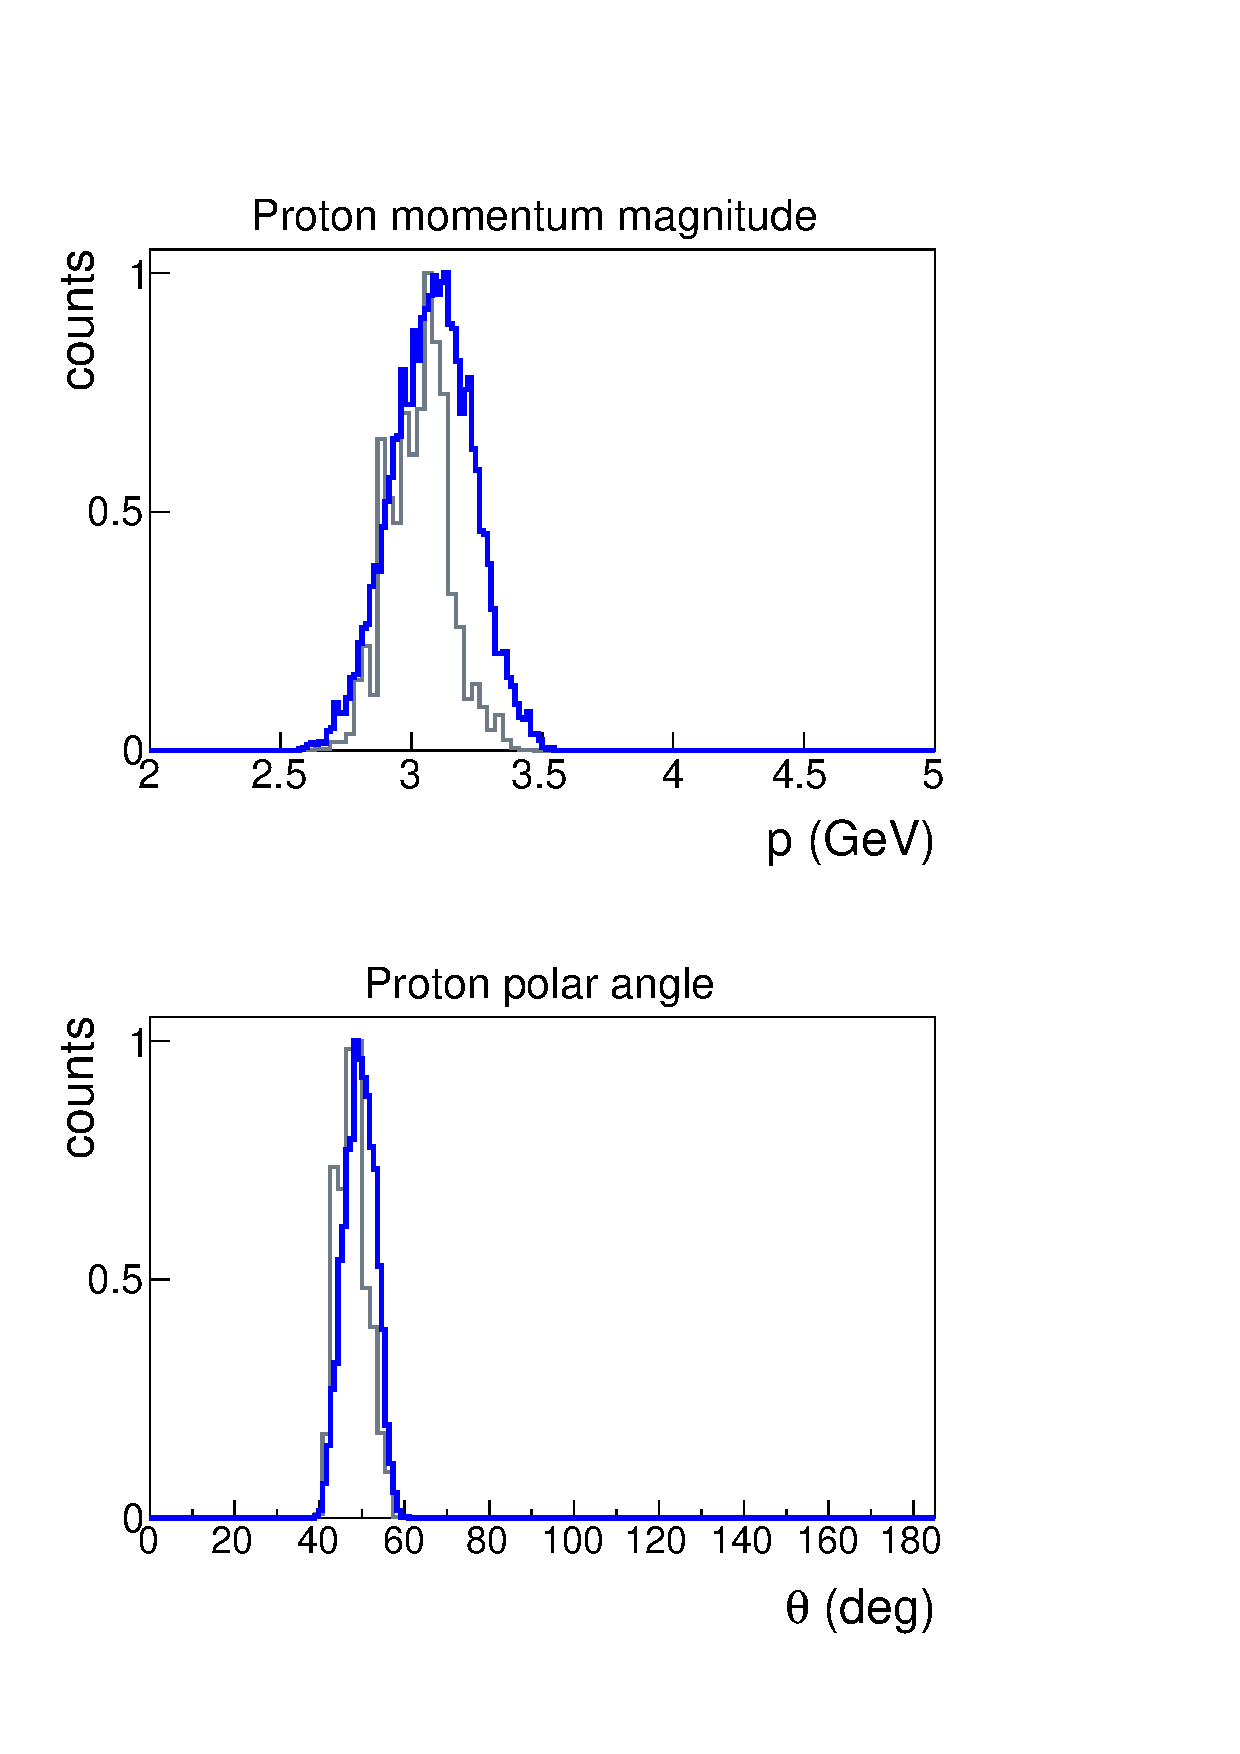
\includegraphics[width=8.2cm]{pictures/generated_p.pdf}
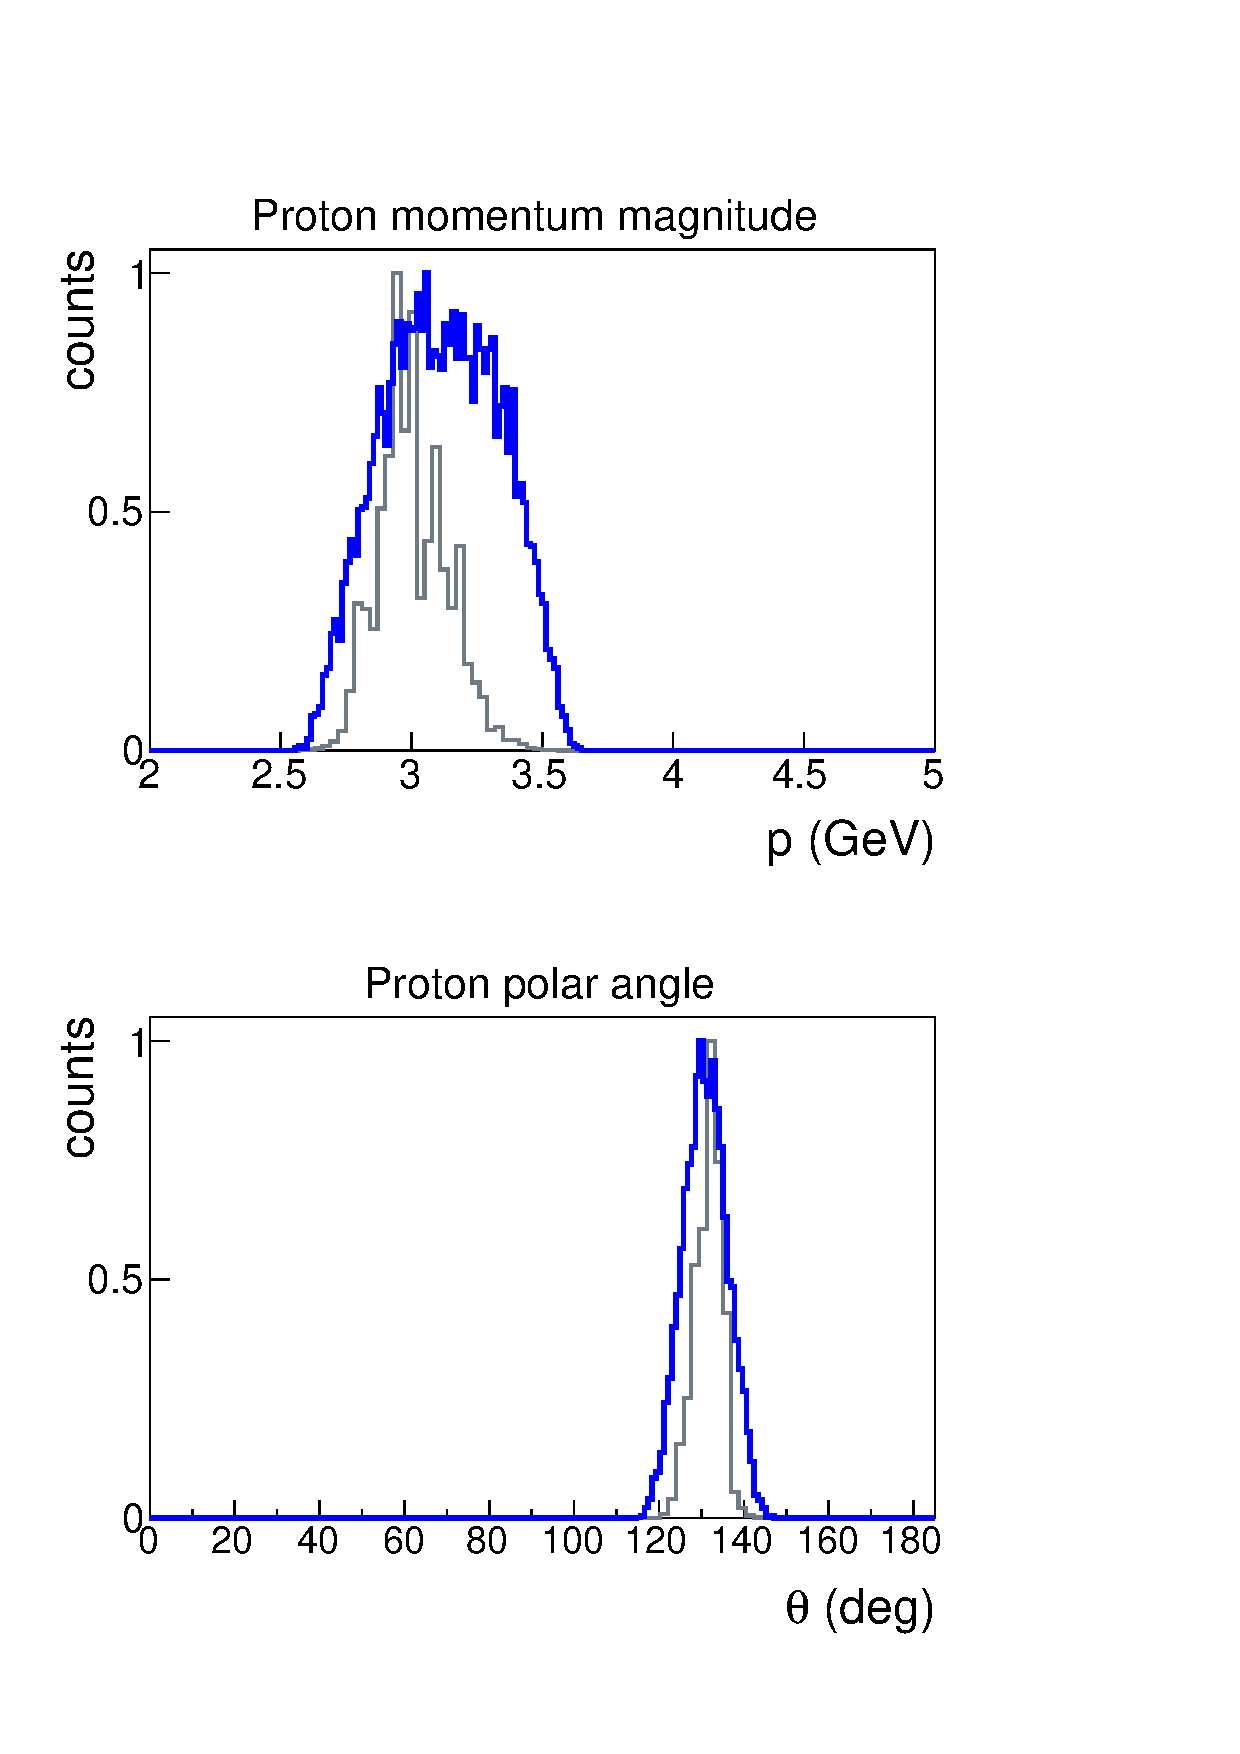
\includegraphics[width=8.2cm]{pictures/generated_pp.pdf}
\caption{\small  Distributions of the momentum magnitude (top row) and the polar angle (bottom row) for the two final protons. The left plots correspond to the proton $p_{3}$ and the right plots -- to the proton $p_{4}$ (as denoted in Fig.~\ref{fig:diagram}). Thick blue histograms correspond to the unweighted distributions and thin background histograms show the distributions weighted with the ``GEA" cross section approximation (see Ch.~\ref{chapter_rate} for details). The simulation was performed in the following kinematic area, $\sqrt{s}=13$~GeV, $\alpha_{s} =1$ with $\Delta \alpha_{s} = 0.25$, $t=-6.8$~GeV$^2$ (which corresponds to $\theta_{\textrm{c.m.}}=49^{o}$) with $\Delta t = 2.5$~GeV$^{2}$, $\Delta \phi = 2\pi$, and $0.1$~GeV/c~$<p_{st}<0.5$~GeV/c. All histograms are normalized to their maxima.} \label{fig:gen_protons}
\end{center}
\end{figure}

\newpage
\begin{figure}[htp]
\begin{center}
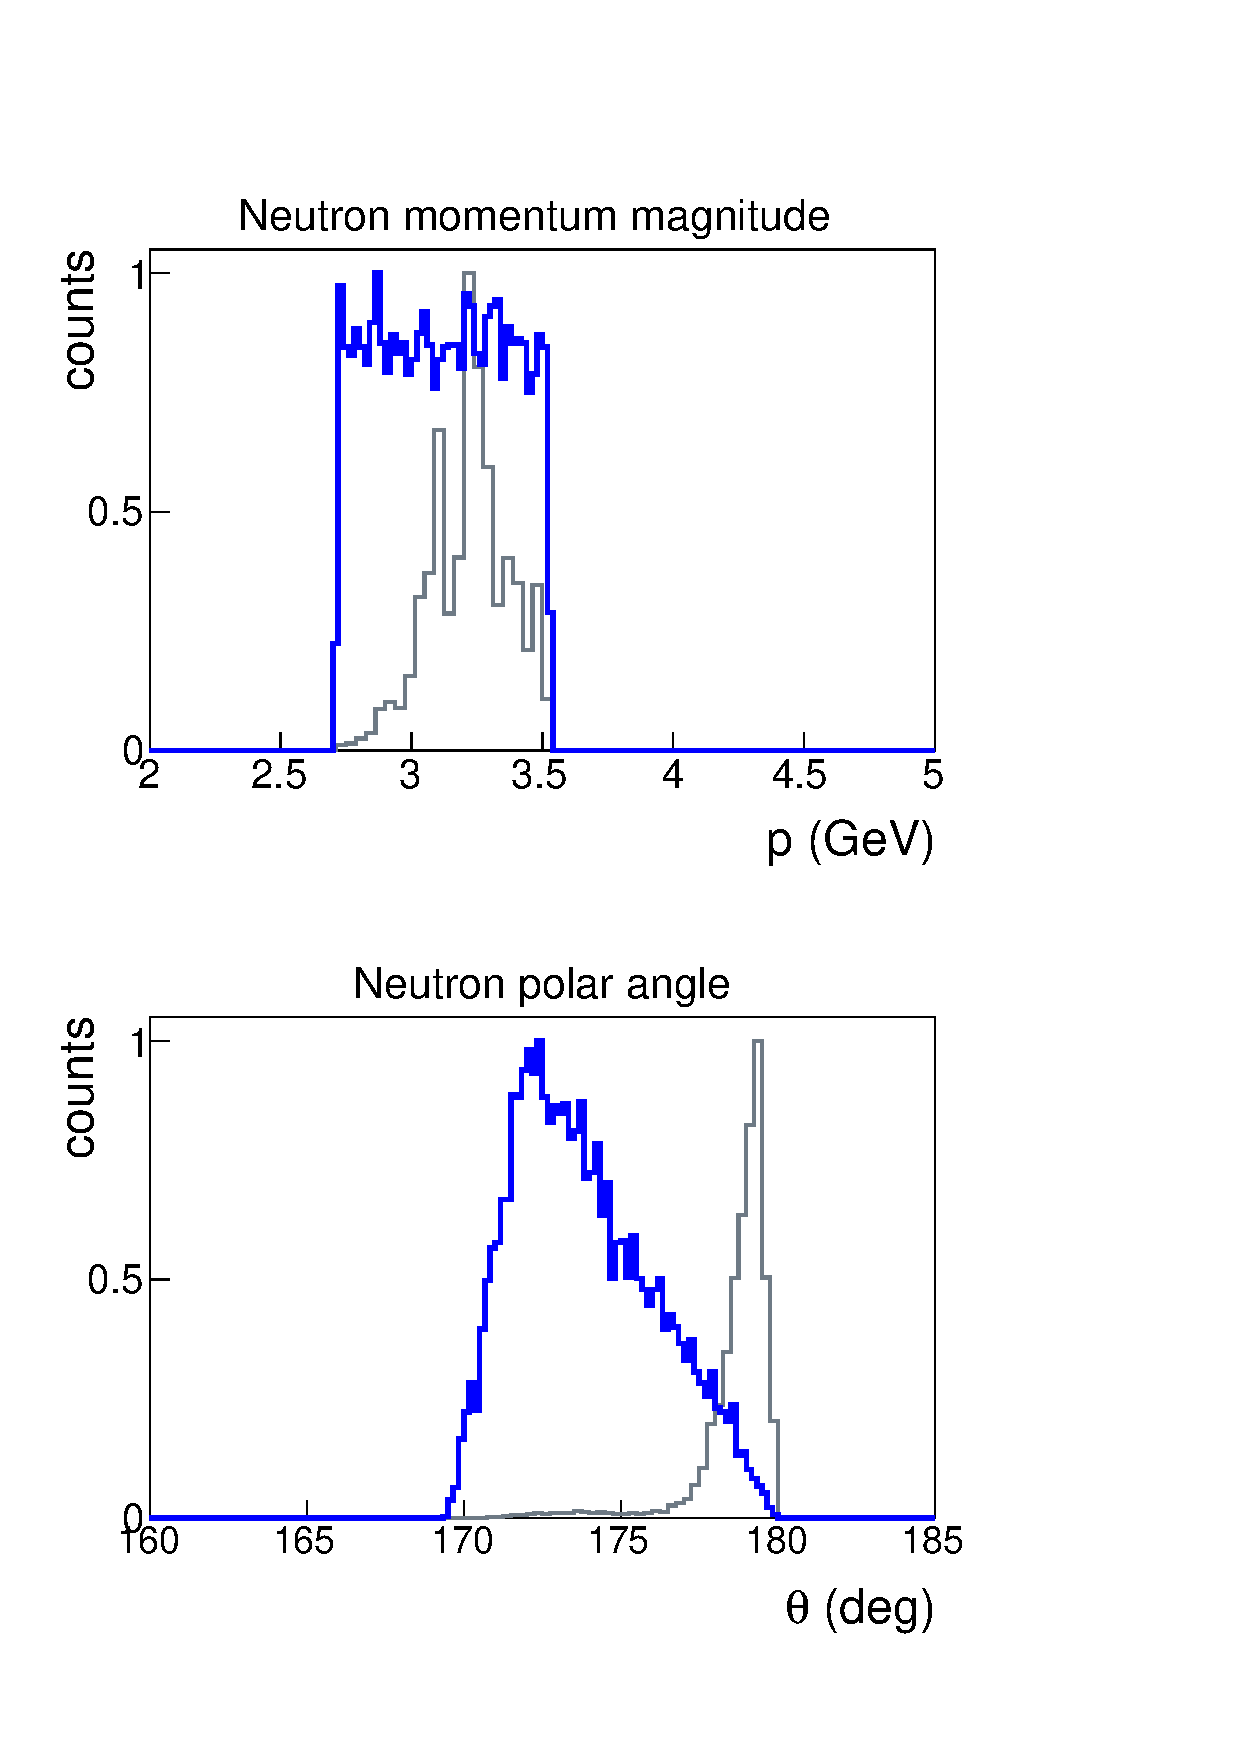
\includegraphics[width=8.2cm]{pictures/generated_nn.pdf}
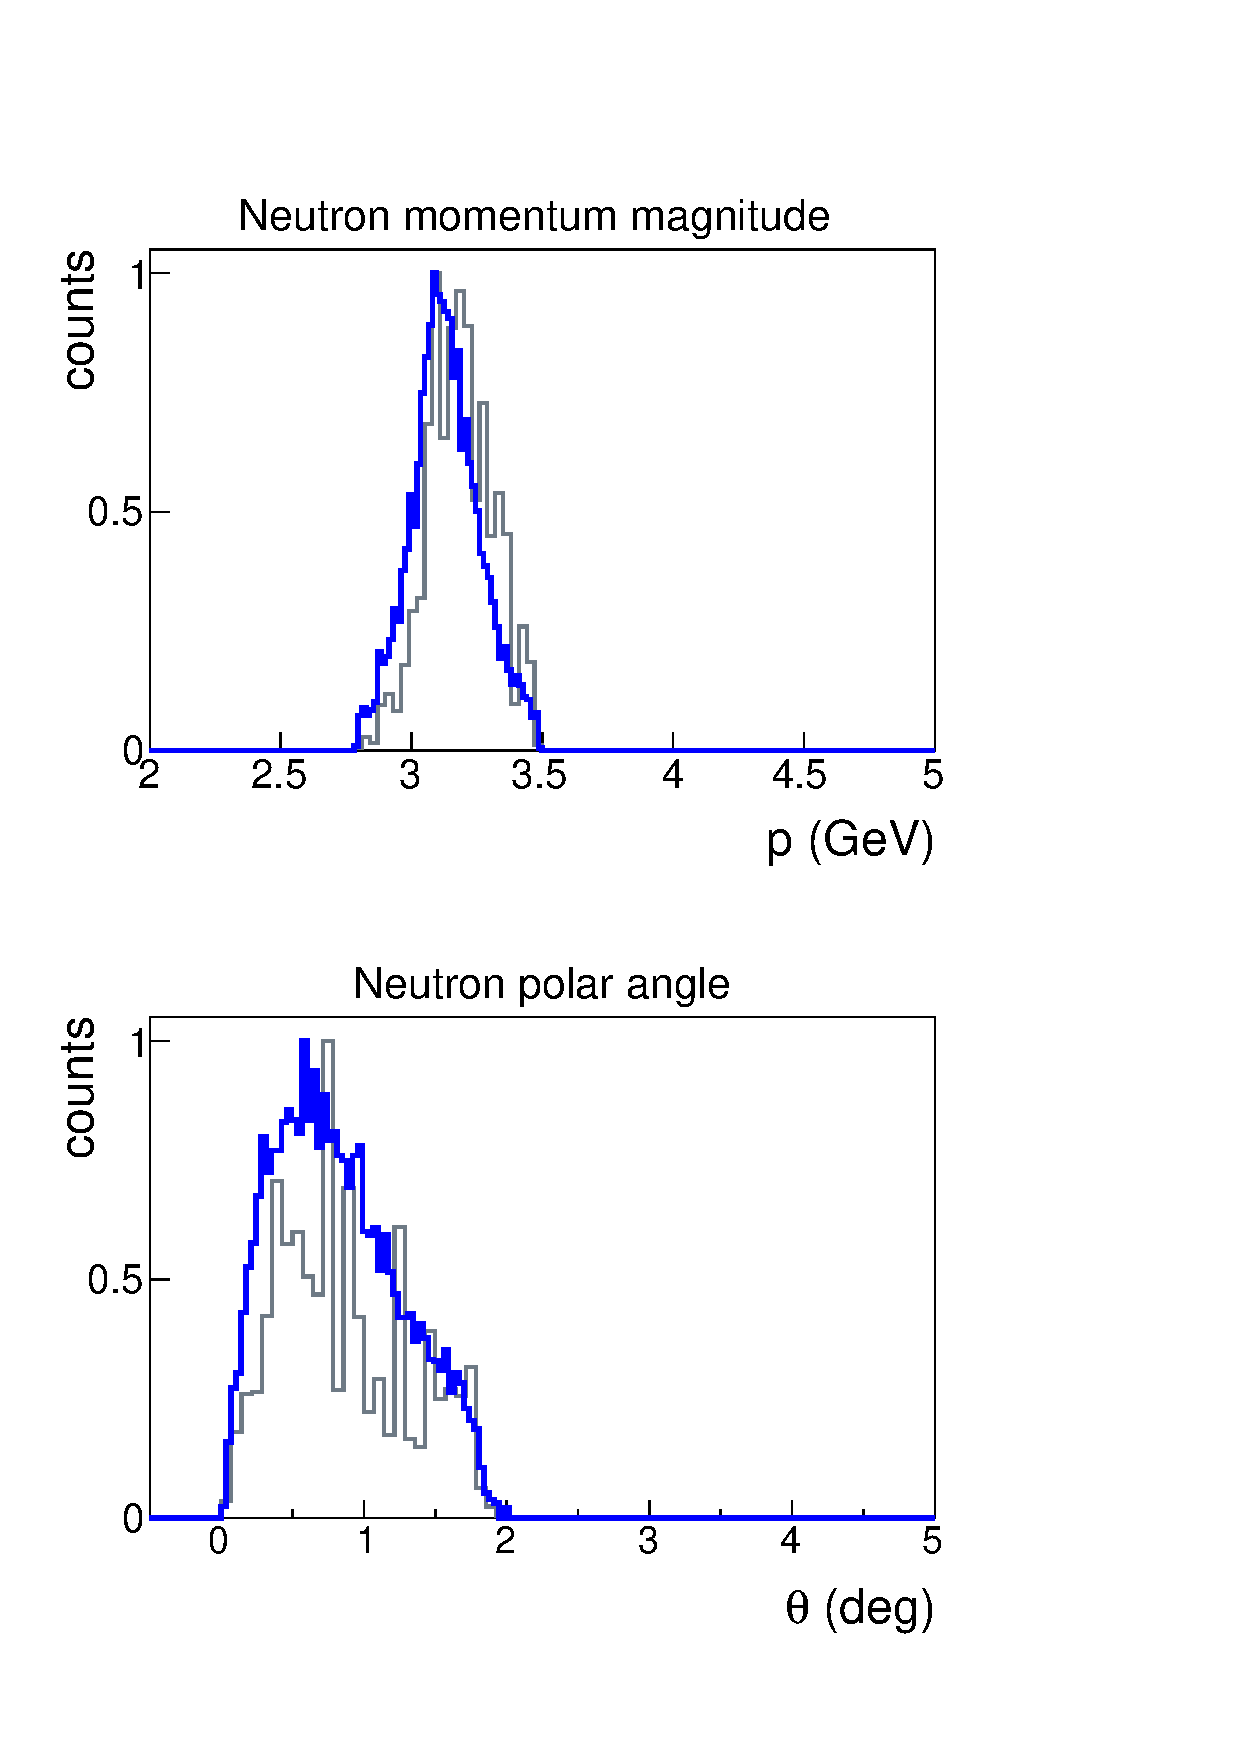
\includegraphics[width=8.2cm]{pictures/generated_n.pdf}
\caption{\small  Distributions of the momentum magnitude (top row) and the polar angle (bottom row) for the two final neutrons. The left plots correspond to the neutron $p_{s}$ and the right plots -- to the neutron $p_{s1}$ (as denoted in Fig.~\ref{fig:diagram}). Thick blue histograms correspond to the unweighted distributions and thin background histograms show the distributions weighted with the ``GEA" cross section approximation (see Ch.~\ref{chapter_rate} for details). The simulation was performed in the following kinematic area, $\sqrt{s}=13$~GeV, $\alpha_{s} =1$ with $\Delta \alpha_{s} = 0.25$, $t=-6.8$~GeV$^2$ (which corresponds to $\theta_{\textrm{c.m.}}=49^{o}$) with $\Delta t = 2.5$~GeV$^{2}$, $\Delta \phi = 2\pi$, and $0.1$~GeV/c~$<p_{st}<0.5$~GeV/c. All histograms are normalized to their maxima.} \label{fig:gen_neutrons}
\end{center}
\end{figure}
\newpage

Figure~\ref{fig:gen_protons} presents event distributions of the momentum magnitude (top row) and the polar angle (bottom row) for the two final protons. The left plots correspond to the proton $p_{3}$ and the right plots -- to the proton $p_{4}$ (as denoted in Fig.~\ref{fig:diagram}). Thick blue histograms correspond to the unweighted distributions and thin background histograms show the distributions weighted with the ``GEA" cross section approximation (see Ch.~\ref{chapter_rate} for details). All histograms are normalized to their maxima. 

As seen in the bottom left plot in Fig.~\ref{fig:gen_protons}, the polar angle of the proton $p_{3}$ peaks at around 50$^o$, which corresponds to the kinematic point where the event generation was performed ($\theta_{\textrm{c.m.}}=49^{o}$ that corresponds to $t=-6.8$~GeV$^2$). Another proton ($p_{4}$) goes in the opposite direction (meaning that the sum of the polar angles of the two protons is equal to $\pi$). Note that in the experiment, only quasi-free protons will follow this back-to-back pattern, while the protons involved in soft rescattering off the reaction neutron $p_{s}$ will acquire disturbed kinematics.

Figure~\ref{fig:gen_neutrons} presents event distributions of the momentum magnitude (top row) and the polar angle (bottom row) for the two final neutrons. The left plots correspond to the neutron $p_{s}$ and the right plots -- to the neutron $p_{s1}$ (as denoted in Fig.~\ref{fig:diagram}). Thick blue histograms correspond to the unweighted distributions and thin background histograms show the distributions weighted with the ``GEA" cross section approximation (see Ch.~\ref{chapter_rate} for details). All histograms are normalized to their maxima. 

The neutron $p_{s}$ (left plots in Fig.~\ref{fig:gen_neutrons}) is assumed to be a spectator to the proton knock-out process $pd \rightarrow ppn$. This neutron ($p_{s}$) goes in the backward direction (its polar angle is close to $\pi$). Another neutron ($p_{s1}$), which is assumed to be a spectator to the entire $p-d$ collision, goes in the forward direction (right plots in Fig.~\ref{fig:gen_neutrons}). For this neutron ($p_{s1}$), both maximal transverse momentum and maximal absolute value of the longitudinal momentum in the $d_{1}$ reference frame were set to 0.1 GeV/c during the event generation. These cuts (which preserve about 75\% of the deuteron momentum distribution) were needed to exclude the rescattering of the $p_{s1}$ neutron, thus ensuring it to be a spectator to the investigated $p-d$ collision. 

It should be emphasized that in Fig.~\ref{fig:gen_neutrons}, the kinematic distributions for the neutrons $p_{s}$ and $p_{s1}$ differ mainly because in the event generator the $p_{s1}$ neutron is assumed to be quasi-free (as described above). However, in the experiment, kinematic distributions of both neutrons will be indistinguishable from each other.

For the bottom left plot in Fig.~\ref{fig:gen_neutrons}, a remarkably large difference between the weighted and unweighted event distributions is observed. This seems to be due to a very steep cross section drop with $p_{st}$ (as seen e.g. in Fig.~\ref{fig:model}) and the fact that the $p_{st}$ value and the neutron polar angle are correlated. Therefore, smaller neutron polar angles (in the lab frame) correspond to the region with a very low cross section and vice versa.


%Note that all event distributions in Figs.~\ref{fig:gen_protons} and~\ref{fig:gen_neutrons} are Fermi smeared and the Fermi momentum in the event generator was generated according to the Paris potential~\cite{Lacombe:1981eg}.


Also note that other available cross section approximations (``IA" and ``CT"), when used as weights for kinematic distributions presented in Figs.~\ref{fig:gen_protons} and~\ref{fig:gen_neutrons}, resulted in histograms almost indistinguishable from the case when the ``GEA" approximation was used (and for this reason only the ``GEA" histograms are shown in the plots).  



